\documentclass{article}

\usepackage[utf8]{inputenc}
\usepackage{amsmath,amssymb,amsthm}
\usepackage{algorithm}
\usepackage{algorithmic}
\usepackage{booktabs}
\usepackage{graphicx}
\usepackage{hyperref}
\usepackage{microtype}
\usepackage[margin=1in]{geometry}
\graphicspath{{../figures/}{figures/}}

\newtheorem{theorem}{Theorem}
\newtheorem{proposition}[theorem]{Proposition}
\DeclareMathOperator{\tr}{tr}
\DeclareMathOperator{\rank}{rank}
\newcommand{\R}{\mathbb{R}}
\newcommand{\E}{\mathbb{E}}
\newcommand{\bW}{\mathbf{W}}
\newcommand{\bM}{\mathbf{M}}
\newcommand{\bC}{\mathbf{C}}
\newcommand{\bU}{\mathbf{U}}
\newcommand{\bV}{\mathbf{V}}
\newcommand{\bSigma}{\mathbf{\Sigma}}

\title{\textbf{Hetero}: Activation-Aware Conditional-Expert\\
Neural Network Inheritance}
\author{Anonymous Authors}
\date{}

\begin{document}
\maketitle

\begin{abstract}
Hetero turns fixed-capacity neural-network inheritance into a
preserve-then-adapt initialization.  At the exact InherNet rank and parameter
count, it minimizes activation-weighted local reconstruction error for the
inherited expert mean, then introduces zero-sum expert deviations that preserve
this reconstruction while exposing conditional router directions.  A
zero-step study on Oxford Pets and CIFAR-100 verifies both predicted effects:
activation weighting improves teacher-behavior preservation at fixed capacity,
and the conditional lift activates every measured router without changing the
inherited task metric or teacher agreement.  Hetero thereby connects
task-relevant preservation and conditional adaptation through one constrained
initialization rather than additional capacity or rank reallocation.
\end{abstract}

\section{Motivation and Contributions}

Weight-space SVD preserves dominant parameters, but not necessarily behavior
on task-relevant activations.  Moreover, identical inherited experts make the
router locally insensitive at initialization.  Hetero addresses both
limitations through one constrained construction:
\begin{enumerate}
  \item the expert-mean operator is selected under the empirical activation
        metric; and
  \item expert deviations are introduced in its zero-sum subspace, preserving
        the inherited mean while making conditional routing locally trainable.
\end{enumerate}
This construction provides exact capacity matching, a closed-form local optimum
under the empirical activation metric, and reconstruction-preserving
conditional directions.

Activation-oriented decomposition is established by SVD-LLM
\cite{wang2025svdllm} and CorDA \cite{yang2024corda}, while LEMON
\cite{wang2024lemon} provides a precedent for symmetry-preserving model
transformation.  Hetero's contribution is the inheritance-specific
preserve-then-adapt constraint that connects these principles at fixed
conditional-expert capacity.

\section{InherNet Baseline and Trained Sources}

For a trained source weight $\bW\in\R^{m\times n}$ with
$\bW=\bU\bSigma\bV^\top$, the rank-$r$ InherNet initialization is
\begin{equation}
  \bW^{\mathrm{down}}=\bSigma_r^{1/2}\bV_r^\top,
  \qquad
  \bW_h^{\mathrm{up}}=\bU_r\bSigma_r^{1/2}.
  \label{eq:inher-init}
\end{equation}
The softmax gate sums to one, so identical up-projection experts reconstruct
$\bU_r\bSigma_r\bV_r^\top$ at initialization.  All methods inherit from the
same task-trained dense checkpoint.  The source remains frozen when used for
distillation, ensuring that differences arise from the inherited
parameterization and training objective rather than teacher drift.

\section{Hetero Method}

\subsection{Uncentered Activation Second Moments}

For a layer input feature $x$, Hetero estimates
\begin{equation}
  \widehat{\bM}=\frac{1}{N}\sum_{i=1}^{N}x_ix_i^\top.
  \label{eq:second-moment}
\end{equation}
The uncentered second moment follows directly from the local objective
\begin{equation}
  \E\| (\bW-\widehat{\bW})x\|_2^2
  =\tr\!\left((\bW-\widehat{\bW})\bM
              (\bW-\widehat{\bW})^\top\right).
  \label{eq:local-error}
\end{equation}
The empirical estimate is stabilized using
\begin{equation}
  \mu=\frac{\tr(\widehat{\bM})}{d},\qquad
  \bM_\lambda=(1-\lambda)\widehat{\bM}
  +\lambda\mu\mathbf{I}+\epsilon\mu\mathbf{I}.
  \label{eq:shrinkage}
\end{equation}
The reference configuration uses $\lambda=0.01$, 16 calibration batches, and
at most 4096 sampled features per layer and batch.  Matrix-valued modes add
positive diagonal jitter before Cholesky factorization; we write
$\widetilde{\bM}_\lambda$ for the stabilized matrix actually factored.

Calibration scales with layer shape.  Convolution patch dimensions up to 256
use exact unfolded patch moments, while wider convolutions use a stride-,
dilation-, padding-, and kernel-position-aware channel-block approximation.
Linear input dimensions up to 512 use a full second moment, while wider linear
layers use a diagonal moment.  Transformer padding tokens are excluded using
the attention mask.  The full-moment construction instantiates the theorem in
Section~\ref{sec:theory} exactly; channel-block and diagonal statistics define
memory-bounded surrogate metrics.

\subsection{Data-Weighted Preserve-Then-Adapt Decomposition}

Let
\begin{equation}
  \widetilde{\bM}_\lambda=\bC\bC^\top,
  \qquad \bA=\bW\bC.
  \label{eq:weighted-operator}
\end{equation}
For $[\bA]_r=\bU_r\bSigma_r\bV_r^\top$, Hetero initializes
\begin{align}
  \bW^{\mathrm{down}}
    &=\bSigma_r^{1/2}\bV_r^\top\bC^{-1},
    \label{eq:hetero-down}\\
  \bW_h^{\mathrm{up}}
    &=\bU_r\bSigma_r^{1/2}+\bE_h,
    \qquad \sum_{h=1}^{H}\bE_h=\mathbf{0}.
    \label{eq:hetero-up}
\end{align}
The first constraint preserves the source where calibration activations place
mass.  The second breaks expert symmetry without changing the average
reconstruction.  A zero-initialized softmax router consumes the compressed
feature, so the two constraints form one preserve-then-adapt initialization.

\subsection{Registered-Rank Capacity Matching}

Hetero uses the same registered layer rank, eligible layers, expert count,
router dimensions, biases, and dense-layer decisions as its matched InherNet.
Hetero-Lite matches InherNet-Small, while Hetero matches InherNet-Large.
Consequently, each comparison has exact total-model parameter equality by
construction, including fixed vision parameters and fixed BERT embeddings.

The CIFAR-100 pairs use the ranks printed in the InherNet paper.  Measured
construction counts are reported for the two pairs whose printed ranks and
reported counts disagree.  Hetero fixes these registered ranks by design.  The
pre-study evaluates heterogeneous allocation under the same parameter cap only as a
diagnostic of whether additional allocation complexity improves behavioral
preservation.

\subsection{Routing and Training Objective}

For mean routing probabilities $\bar g_h$, define
\begin{equation}
  \mathcal{L}_{\mathrm{bal}}
  =H\sum_{h=1}^{H}\bar g_h^2-1\geq0.
  \label{eq:balance}
\end{equation}
The current reference fine-tuning objective uses
$\lambda_{\mathrm{bal}}=0.01$:
\begin{equation}
  \mathcal{L}
  =w_{\mathrm{CE}}\mathcal{L}_{\mathrm{CE}}
   +w_{\mathrm{KD}}T^2
     \operatorname{KL}(p_{\mathrm{teacher}}^T
                        \|p_{\mathrm{student}}^T)
   +\lambda_{\mathrm{bal}}\mathcal{L}_{\mathrm{bal}}.
  \label{eq:training-objective}
\end{equation}
For supervised configurations, the task term replaces the CE--KD mixture.
HPO compares $\lambda_{\mathrm{bal}}\in\{0,0.01,0.03\}$, and the zero-weight
component ablation isolates its contribution.  All inherited factors and
routers are optimized end to end.

\begin{algorithm}[t]
\caption{Hetero registered-rank decomposition}
\label{alg:hetero}
\begin{algorithmic}[1]
\REQUIRE Trained source; calibration loader; registered rank; number of
heads; moment and perturbation settings.
\FOR{each eligible layer $l$}
  \STATE Estimate the regularized uncentered second moment with the applicable
         full, channel-block, or diagonal mode.
  \STATE Factor $\bM_l=\bC_l\bC_l^\top$ and compute the SVD of
         $\bW_l\bC_l$.
  \STATE At the registered rank, construct
         Eqs.~\eqref{eq:hetero-down}--\eqref{eq:hetero-up}; retain the same
         dense layers as matched InherNet.
\ENDFOR
\STATE Attach a zero-initialized compressed-feature router and verify exact
       parameter equality with matched InherNet.
\STATE Train inherited factors and routers end to end.
\end{algorithmic}
\end{algorithm}

\section{Theoretical Analysis}
\label{sec:theory}

\subsection{Data-Weighted Eckart--Young Theorem}

\begin{theorem}[Data-weighted Eckart--Young--Mirsky]
Let $\bM\succ0$, $\bM=\bC\bC^\top$, and $\bA=\bW\bC$.  Among all matrices
$\bQ$ with $\rank(\bQ)\leq r$,
\begin{equation}
  \bQ_r^*=[\bA]_r\bC^{-1}
\end{equation}
minimizes
\begin{equation}
  \tr\!\left((\bW-\bQ)\bM(\bW-\bQ)^\top\right)
  =\|(\bW-\bQ)\bC\|_F^2.
\end{equation}
\end{theorem}

\begin{proof}
Set $\bB=\bQ\bC$.  Invertibility of $\bC$ preserves rank, and the objective
becomes $\|\bA-\bB\|_F^2$.  The ordinary Eckart--Young--Mirsky theorem
\cite{eckart1936approximation} gives
$\bB^*=[\bA]_r$, hence $\bQ_r^*=[\bA]_r\bC^{-1}$.
\end{proof}

\subsection{Initialization Preservation and Conditional Tangent}

\begin{proposition}[Initialization preservation]
With a zero-initialized softmax router and perturbations satisfying
$\sum_h\bE_h=0$, the mean expert map at initialization equals
$[\bW\bC]_r\bC^{-1}$ up to numerical error.
\end{proposition}

\begin{proof}
The zero-initialized router gives $g_h=1/H$.  Substituting
Eqs.~\eqref{eq:hetero-down}--\eqref{eq:hetero-up} and averaging eliminates
$\sum_h\bE_h$, leaving
$\bU_r\bSigma_r\bV_r^\top\bC^{-1}$.
\end{proof}

Let $z=\bW^{\mathrm{down}}x$, write expert $h$ as $\bB+\bE_h$, and let $a_j$
denote router logit $j$.  At the same initialization,
\begin{equation}
  \frac{\partial y}{\partial a_j}
  =g_j\big((\bB+\bE_j)z+b-y\big)
  =\frac{1}{H}\bE_jz.
  \label{eq:router-gradient}
\end{equation}
Identical experts give a zero router derivative at the zero-logit
initialization; the zero-sum lift generically exposes a first-order conditional
learning signal while preserving the inherited map.

\subsection{From Local Guarantee to Empirical Evaluation}

The theorem identifies the layer-local behavior guaranteed by the construction.
It is exact for the stabilized full moment, while channel-block and diagonal
statistics provide scalable surrogate metrics.  Sections 6 and 7 connect these
initialization properties to downstream accuracy and learned specialization
through controlled empirical evaluation.

\section{Dataset and Model Protocols}

\begin{table}[t]
\centering
\small
\resizebox{\textwidth}{!}{%
\begin{tabular}{@{}lllll@{}}
\toprule
Family & Teacher $\rightarrow$ student & Initialization & Source/objective & Targets \\
\midrule
CIFAR-10 & ResNet-50 $\rightarrow$ ResNet-18, CIFAR stem
  & random & trained teacher / KD & convolution \\
CIFAR-100 & eight native ResNet, VGG, WRN pairs
  & random & trained teacher / supervised & convolution \\
Oxford-IIIT Pet & ResNet-34 $\rightarrow$ ResNet-18
  & ImageNet pretrained & fine-tuned teacher / KD & convolution \\
GLUE & BERT-Mini $\rightarrow$ BERT-Tiny
  & pretrained compact BERT & fine-tuned teacher / KD & linear \\
\bottomrule
\end{tabular}}
\caption{Dataset, model, and inheritance protocols.}
\label{tab:protocols}
\end{table}

\begin{table}[t]
\centering
\small
\resizebox{\textwidth}{!}{%
\begin{tabular}{@{}lrrrrrl@{}}
\toprule
Family & Optimizer & Batch & Epochs & LR & Weight decay & Schedule \\
\midrule
CIFAR-10 & SGD, mom. 0.9 & 128 & 200 & 0.05 & $5\!\times\!10^{-4}$ & 100/150/180 \\
CIFAR-100 & SGD, mom. 0.9 & 64 & 240 & 0.05 & $5\!\times\!10^{-4}$ & 150/180/210 \\
Oxford-IIIT Pet & SGD, mom. 0.9 & 32 & 30 & 0.001 & $10^{-4}$ & 15/25 \\
GLUE compact BERT & AdamW & 32 & 4 & $5\!\times\!10^{-5}$ & 0.01$^*$ & warmup/linear decay \\
\bottomrule
\end{tabular}}
\caption{Full training schedules.  $^*$Bias and LayerNorm parameters are
excluded from decay; the global gradient norm is clipped at 1.0.}
\label{tab:schedules}
\end{table}

The suite spans scratch-trained vision on CIFAR, ImageNet-initialized
fine-grained transfer on Oxford Pets, and compact-transformer transfer on
GLUE.  Convolutions are inherited for vision, while attention and feed-forward
projections are inherited for GLUE.  The small Oxford classifier, transformer
embeddings, and normalization layers remain dense.  The compact-BERT GLUE
track is a resource-efficient cross-modal extension that complements the
original T5 benchmark \cite{zhou2026inhernet}.

The CIFAR-100 pairs are ResNet-32/8, ResNet-32$\times$4/8$\times$4, VGG-13/8,
WRN-40-2/40-1, WRN-40-2/16-2, ResNet-56/20, ResNet-110/32, and
ResNet-110/20.  GLUE covers MRPC, QQP, SST-2, MNLI, RTE, QNLI, CoLA, and
STS-B.  MRPC and QQP report accuracy and F1; SST-2, MNLI, RTE, and QNLI
report accuracy; CoLA reports Matthews correlation; and STS-B reports Pearson
and Spearman correlations.

\section{Experiment and Search Protocol}

Each teacher is trained for the complete dataset schedule, selected using its
validation metric, and reused unchanged by student KD, InherNet, Hetero,
ablations, and HPO.  CIFAR search uses a fixed stratified 10\% training
holdout, Oxford uses its fixed stratified validation split, and GLUE search
reserves the official validation split for formal reporting.  Official test
data are used only after model selection.

Every HPO candidate uses the same epoch count as formal training.  Mechanism
and learning-rate screening cover CIFAR-10, CIFAR-100
ResNet-56-to-ResNet-20, Oxford Pets, SST-2, and STS-B.  HPO tunes Hetero at
the InherNet-Large capacity; InherNet retains its registered settings, and
Hetero-Lite inherits the selected Hetero recipe as a capacity ablation.

The mechanism screen varies routing regularization, moment shrinkage, and
zero-sum lift scale; learning rate and distillation settings are screened
separately to avoid confounding optimizer and mechanism effects.  Selection
uses seeds 42, 123, and 2026, confirmation uses seed 3407, and final estimates
use disjoint seeds 7, 17, 27, and 37.

For reproducibility, mechanism candidates fix the learning-rate multiplier at
1.0, and mechanism and learning-rate candidates use the objective registered
for each dataset profile.  Distillation candidates likewise fix the multiplier
at 1.0.  These references are read from the committed confirmation registry,
not from recipes selected after HPO; each generated command contains every
controlled argument exactly once.

The comparison includes the teacher, compact student, student KD, and
capacity-matched InherNet under both its registered supervised objective and
the selected Hetero objective.  A supervised Hetero control accompanies every
distilled headline recipe.  Component ablations isolate activation weighting,
the zero-sum conditional lift, learned versus fixed-uniform routing, routing
regularization, and calibration budget.  Hetero-Lite tests the
accuracy--efficiency trade-off.

\section{Problem-Driven Pre-Study}

The pre-study tests two predictions before any optimizer step: activation
weighting should improve teacher-behavior preservation at the same rank and
parameter count, and the zero-sum lift should activate router gradients without
materially changing inherited predictions.  Oxford Pets provides a small,
fine-grained transfer setting; CIFAR-100 ResNet-56-to-ResNet-20 tests transfer
to scratch-trained vision.  Fidelity and task metrics use the complete
validation split.  To isolate local decomposition quality from accumulated
upstream error, a held-out local-operator probe feeds dense-teacher activations
into each matching inherited operator for four deterministic validation
batches and reports the ratio of summed output errors to summed dense-output
energy.  Construction records each layer's relative expert-mean shift to check
the zero-mean lift invariant directly.  Router gradients are measured on the first deterministic
evaluation minibatch---32 Oxford examples or 64 CIFAR-100 examples---using
teacher KL without an optimizer step.  Each router dot reports
$\max(\|\partial\mathrm{KL}/\partial \bW_{\mathrm{gate}}\|_2,
\|\partial\mathrm{KL}/\partial b_{\mathrm{gate}}\|_2)$ for one inherited
layer.

\subsection{Activation Geometry Preserves Task-Relevant Behavior}

At fixed capacity, activation weighting reduces teacher-output relative SSE by
66.52\% on Oxford and 17.59\% on CIFAR-100.  Teacher KL falls by 82.44\% and
14.10\%; agreement rises by 61.41 and 5.28 percentage points.  These
behavioral improvements coincide with gains of 59.175 points in Oxford
balanced accuracy and 4.88 points in CIFAR-100 accuracy.  Output cosine
similarity rises by 0.419 and 0.282.

\begin{figure}[t]
  \centering
  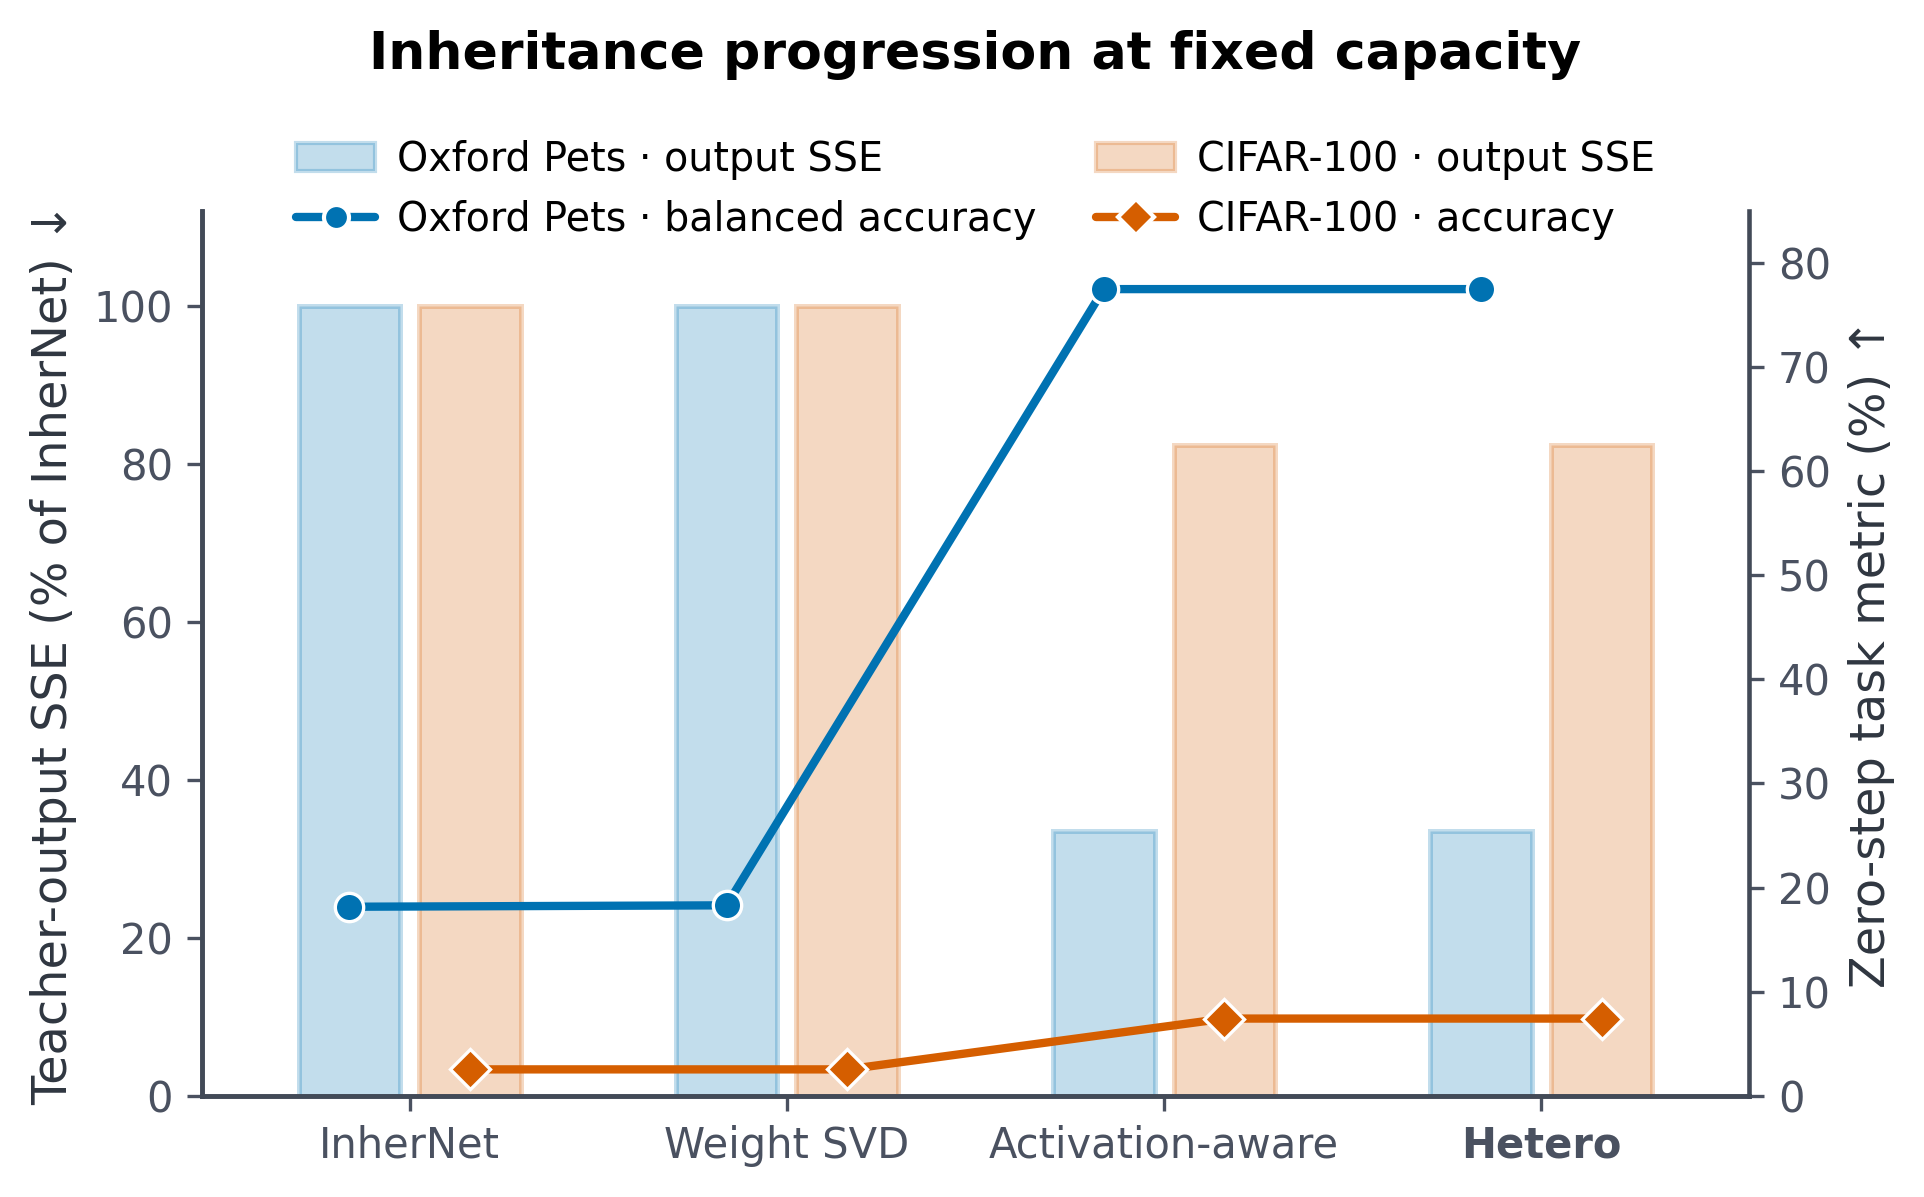
\includegraphics[width=0.82\linewidth]{prestudy_inheritance_progression.png}
  \caption{The fixed-capacity progression isolates activation weighting as
  the source of improved teacher-output fidelity and zero-step task behavior.}
  \label{fig:activation-geometry}
\end{figure}

\subsection{Activation Weighting Improves Every Probed Local Operator}

The held-out local probe isolates each factorized layer by replaying the same
dense-teacher inputs through its dense and inherited operators.  Activation
weighting reduces aggregate local relative SSE from 0.1255 to 0.0598 on Oxford
(52.3\%) and from 0.2869 to 0.1849 on CIFAR-100 (35.6\%).  The improvement
holds for all 65 probed operators across both architectures.  This layerwise
result connects the activation geometry used during decomposition to the
end-to-end behavioral gains above.

\begin{figure}[t]
  \centering
  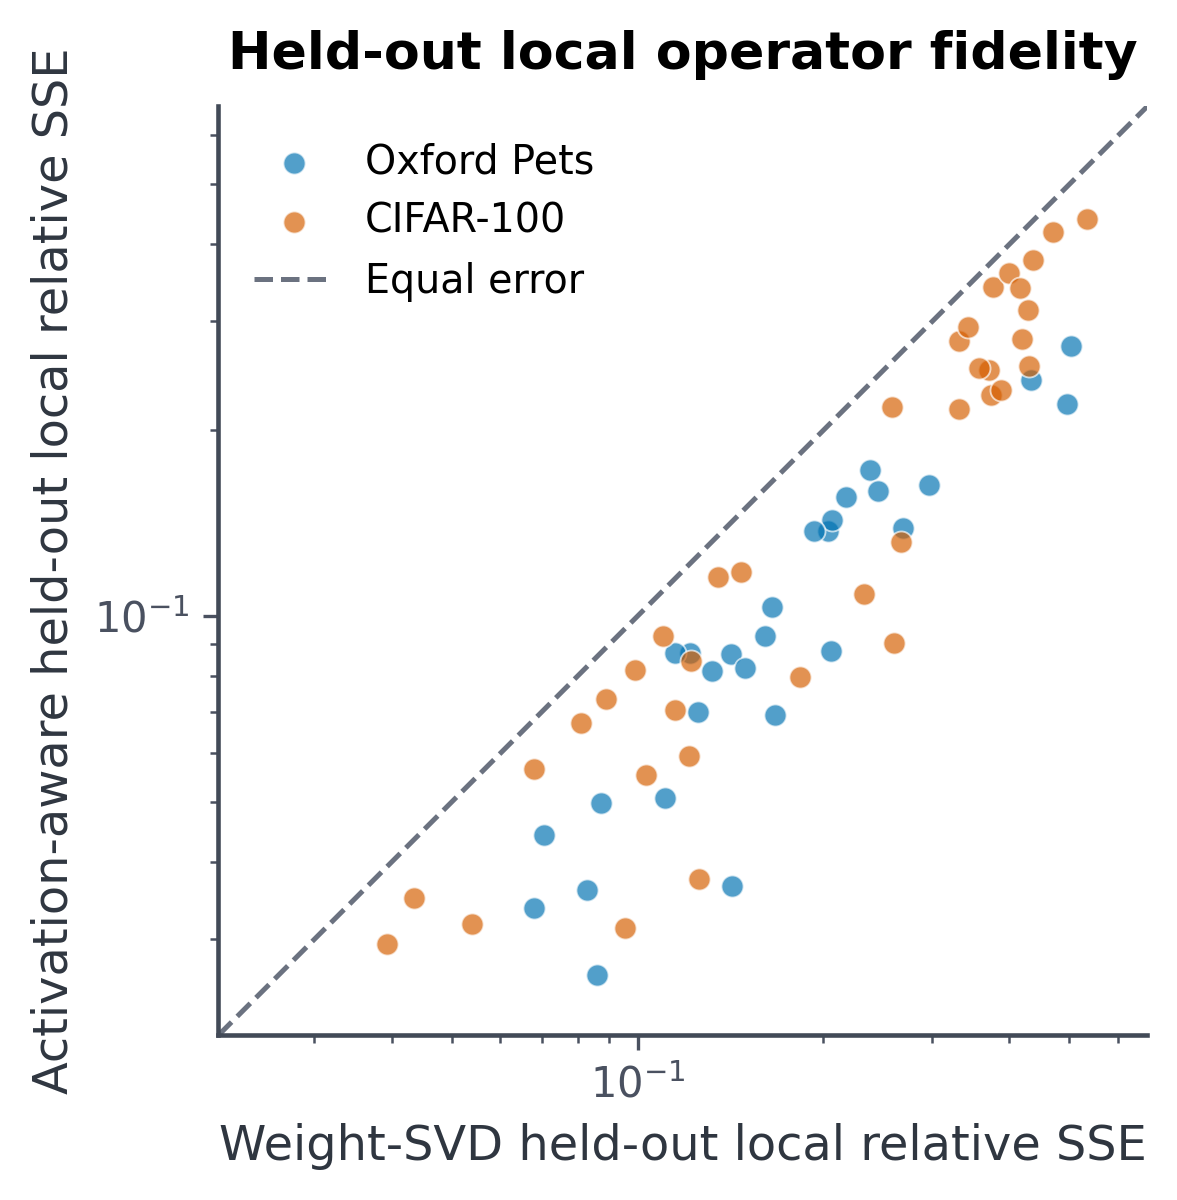
\includegraphics[width=0.68\linewidth]{prestudy_local_operator.png}
  \caption{Activation-aware decomposition lowers held-out local operator
  error for every probed layer on both architectures.}
  \label{fig:local-operator}
\end{figure}

\subsection{The Conditional Lift Exposes Router Tangents}

The zero-sum lift changes relative SSE by only $5.89\!\times\!10^{-5}$ on
Oxford and $1.90\!\times\!10^{-6}$ on CIFAR-100, while leaving task
performance and teacher agreement unchanged.  Normalized routing entropy
remains exactly 1.0, while mean relative expert diversity rises from numerical
zero to 0.008173 on Oxford and 0.008152 on CIFAR-100: the lift creates distinct
experts without disturbing uniform mean routing.  It raises router-gradient RMS
from $1.54\!\times\!10^{-9}$ to $2.27\!\times\!10^{-4}$ on Oxford and from
$3.20\!\times\!10^{-9}$ to $3.63\!\times\!10^{-4}$ on CIFAR-100---about
$1.47\!\times\!10^5$-fold and $1.13\!\times\!10^5$-fold gains.  All 28
Oxford and all 37 CIFAR-100 router layers cross the $10^{-7}$ activity
tolerance after the lift, whereas none cross it with identical experts.

\begin{figure}[t]
  \centering
  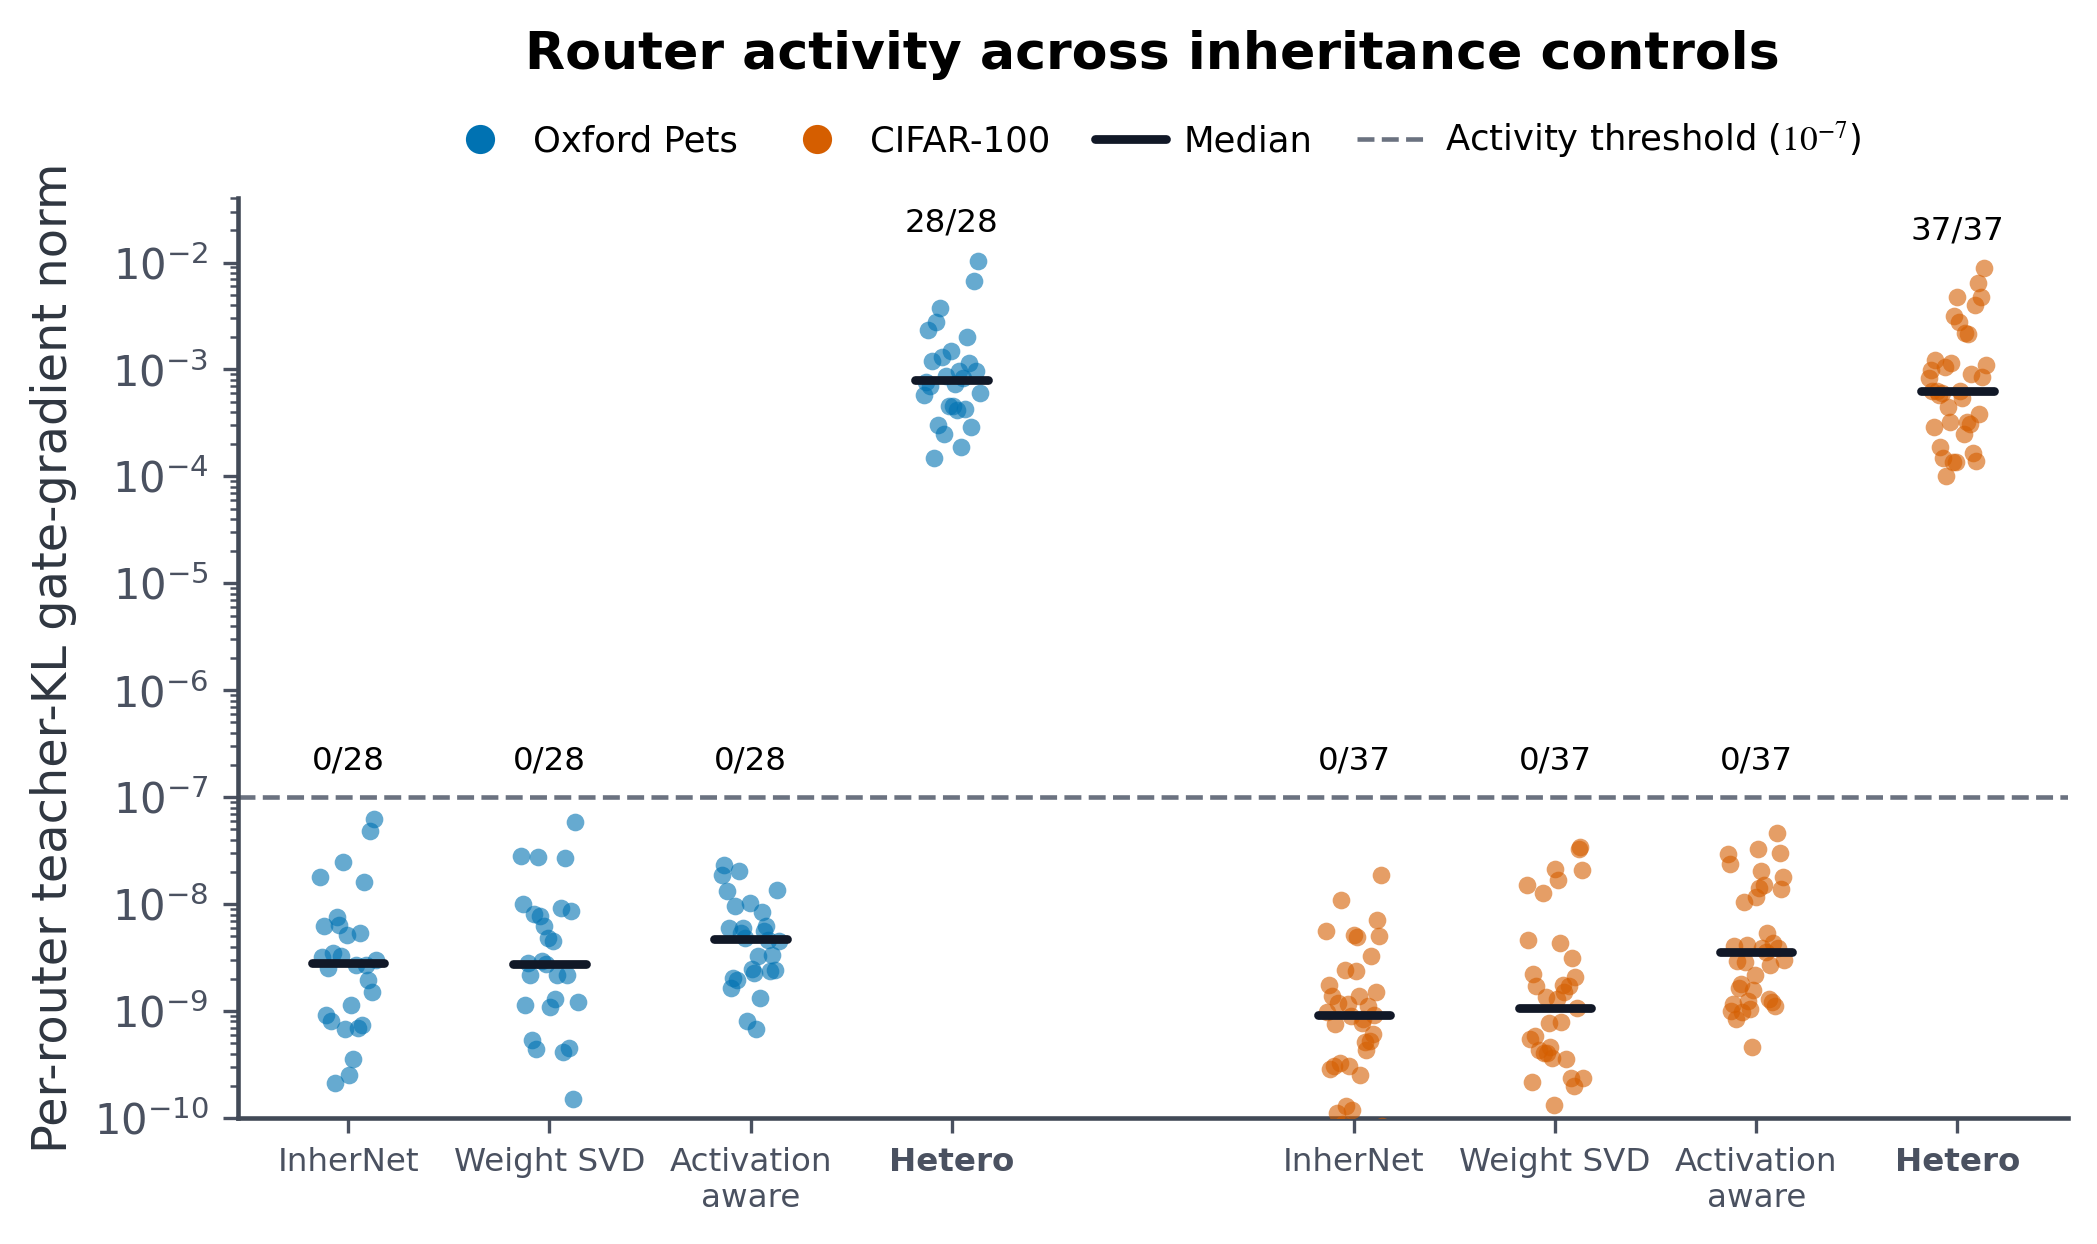
\includegraphics[width=0.88\linewidth]{prestudy_router_activity.png}
  \caption{Only the zero-sum conditional lift activates every measured router
  across the four inheritance controls.}
  \label{fig:router-tangent}
\end{figure}

\subsection{Fixed Rank Avoids a Surrogate--Task Mismatch}

The allocation diagnostic explains why rank reallocation is excluded from the
method.  On CIFAR-100, relative allocation lowers relative SSE from 0.8369 to
0.8108 but also lowers zero-step accuracy from 7.42\% to 6.80\%.  On Oxford,
both relative and nested allocation underperform the fixed-rank
activation-aware construction in reconstruction and balanced accuracy.
Optimizing a layerwise allocation surrogate therefore adds complexity without
reliably improving teacher behavior or the downstream task metric.

\begin{figure}[t]
  \centering
  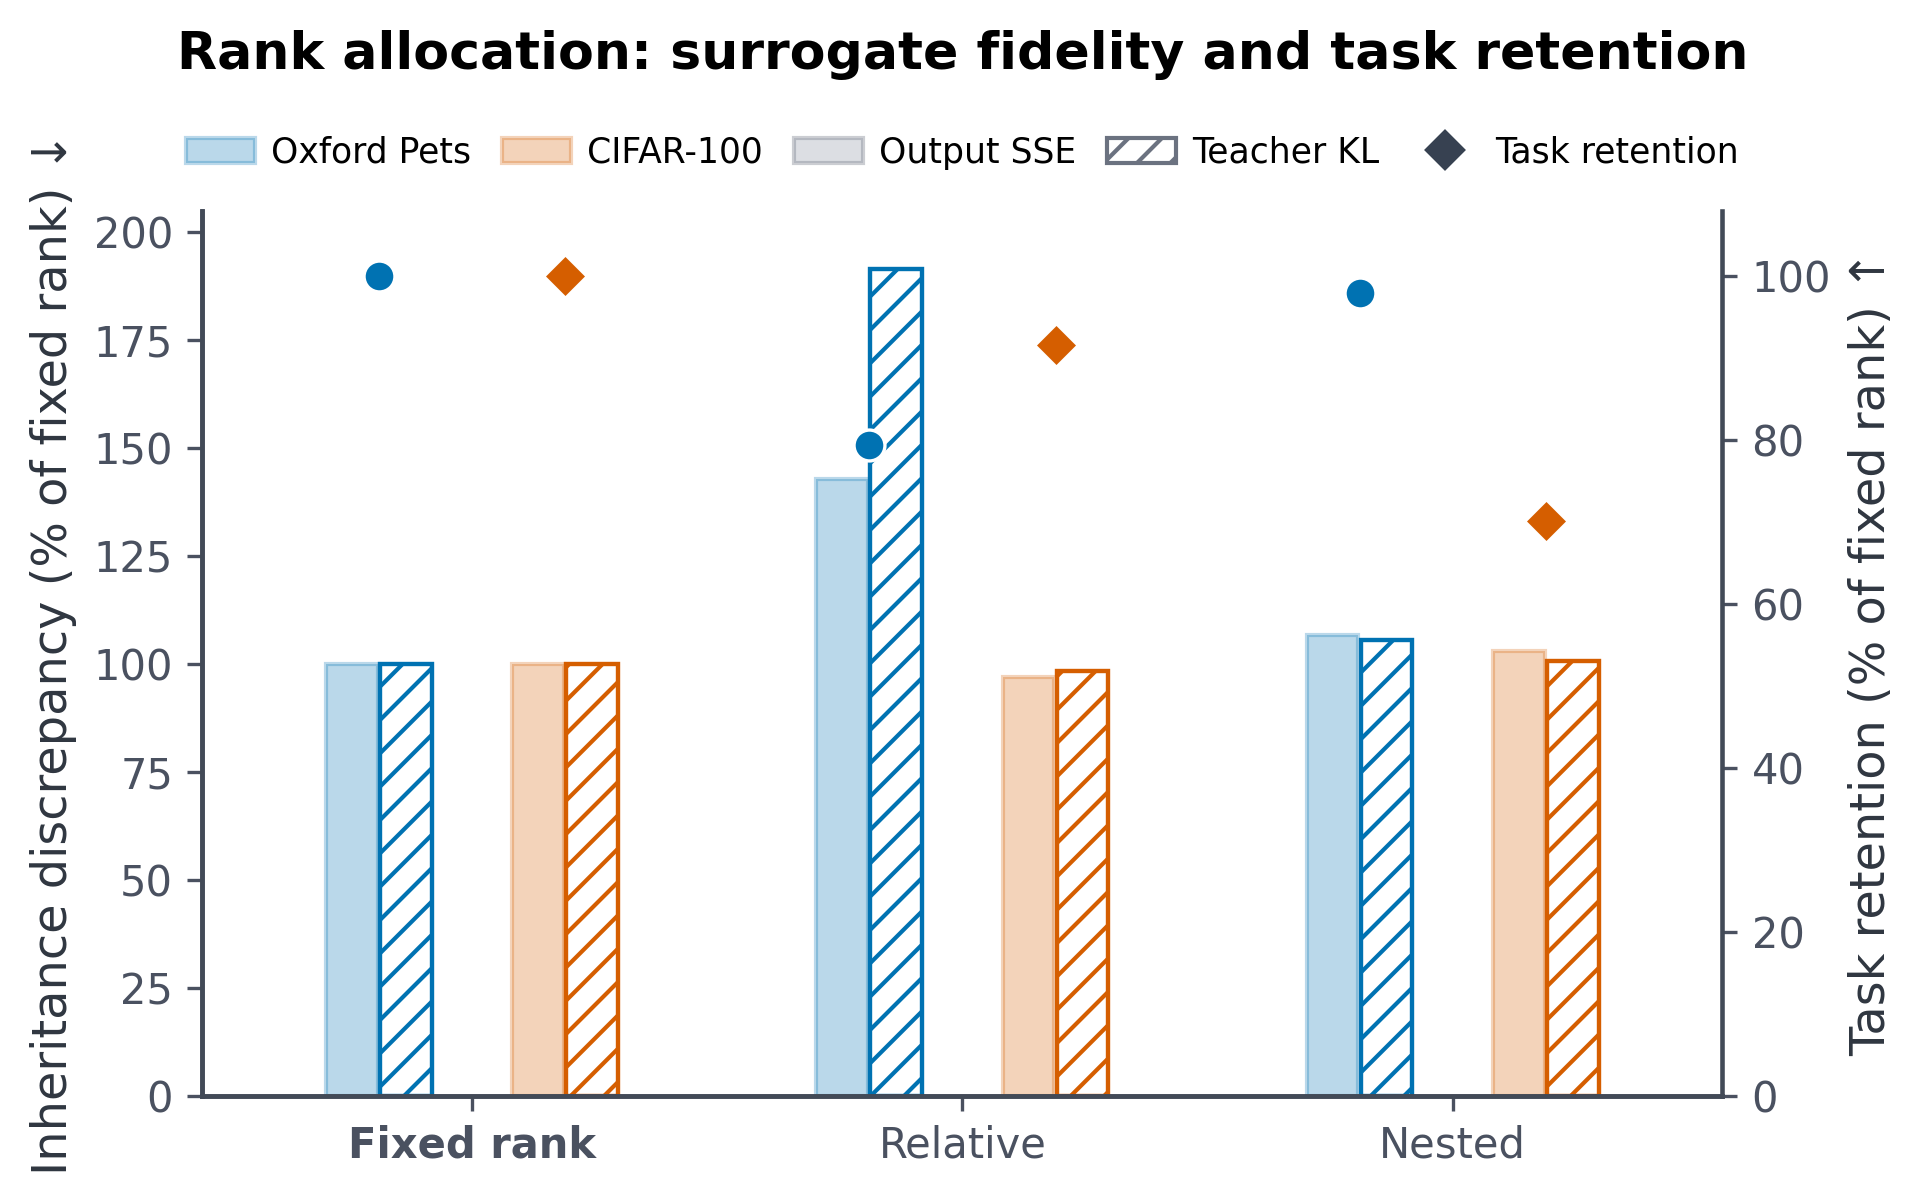
\includegraphics[width=0.82\linewidth]{prestudy_allocation_tradeoff.png}
  \caption{Budget-matched rank allocation can improve output and KL
  surrogates without improving task retention.}
  \label{fig:rank-surrogate}
\end{figure}

\subsection{Completed Zero-Step Diagnostics}

\begin{table}[t]
\centering
\scriptsize
\resizebox{\textwidth}{!}{%
\begin{tabular}{@{}llrlllll@{}}
\toprule
Dataset & Construction & Parameters & Rank & Rel. SSE & KL/agreement & Initial metric & Router RMS \\
\midrule
Oxford & weight-only & 5,699,257 & 64 & .847742 & 2.7661/19.57\% & 18.293 BAcc & $1.63\!\times\!10^{-9}$ \\
Oxford & activation base & 5,699,257 & 64 & .283789 & .4857/80.98\% & 77.468 BAcc & $1.54\!\times\!10^{-9}$ \\
Oxford & Hetero lift & 5,699,257 & 64 & .283848 & .4858/80.98\% & 77.468 BAcc & $2.27\!\times\!10^{-4}$ \\
CIFAR-100 & weight-only & 383,507 & 16 & 1.015533 & 4.3503/2.54\% & 2.54 Acc & $2.36\!\times\!10^{-9}$ \\
CIFAR-100 & activation base & 383,507 & 16 & .836891 & 3.7370/7.82\% & 7.42 Acc & $3.20\!\times\!10^{-9}$ \\
CIFAR-100 & Hetero lift & 383,507 & 16 & .836893 & 3.7368/7.82\% & 7.42 Acc & $3.63\!\times\!10^{-4}$ \\
\bottomrule
\end{tabular}}
\caption{Completed seed-42 zero-step diagnostics.}
\label{tab:diagnostics}
\end{table}

This initialization study establishes the predicted preservation and
conditional-tangent effects; full-epoch, multi-seed experiments will determine
how they translate into the final accuracy--efficiency frontier.

\section{Conclusion}

Hetero recasts inheritance as a constrained initialization problem: preserve
the teacher where task activations place mass, then expose conditional degrees
of freedom without additional capacity or initial reconstruction error.  The
pre-study verifies both predicted initialization effects and motivates a
single, registered-rank preserve-then-adapt mechanism for formal evaluation.

\begin{thebibliography}{9}
\bibitem{zhou2026inhernet}
Y.~Zhou, J.~Shi, M.~Xu, Z.~Jiang, and J.~Chen.
\newblock Beyond Student: An Asymmetric Network for Neural Network Inheritance.
\newblock \emph{arXiv:2602.09509}, 2026.

\bibitem{eckart1936approximation}
C.~Eckart and G.~Young.
\newblock The approximation of one matrix by another of lower rank.
\newblock \emph{Psychometrika}, 1(3):211--218, 1936.

\bibitem{wang2025svdllm}
X.~Wang, Y.~Zheng, Z.~Wan, and M.~Zhang.
\newblock SVD-LLM: Truncation-aware Singular Value Decomposition for Large
Language Model Compression.
\newblock \emph{ICLR}, 2025.

\bibitem{yang2024corda}
Y.~Yang, X.~Li, Z.~Zhou, S.~L. Song, J.~Wu, L.~Nie, and B.~Ghanem.
\newblock CorDA: Context-Oriented Decomposition Adaptation of Large Language
Models for Task-Aware Parameter-Efficient Fine-tuning.
\newblock \emph{NeurIPS}, 2024.

\bibitem{wang2024lemon}
Y.~Wang, J.~Su, H.~Lu, et al.
\newblock LEMON: Lossless Model Expansion.
\newblock \emph{ICLR}, 2024.
\end{thebibliography}

\end{document}
